%!TEX root = ../main.tex

\chapter{評価実験}

\section{予備実験と各種パラメータの決定}\label{sec:lr}

学習率,エポック数等の各種パラメータを決定するために予備実験を行った.

\subsection{RBMの学習率とエポック数}
RBMの学習時の学習率は文献\cite{Hinton-guide}を参考に,更新量が重みの$10^{-3}$程度になるよう決定した.
学習エージェントが実際に採集した,入力を盤面の状態とし,出力を次に石を置く盤面の位置とするデータセットを利用する.RBMの素子数は\ref{sec:node}の自動決定法により決定した.


エポック数とクロスエントロピーの関係を以下の図\ref{fig:ep}に示す.

\begin{figure}[]
\begin{center}
   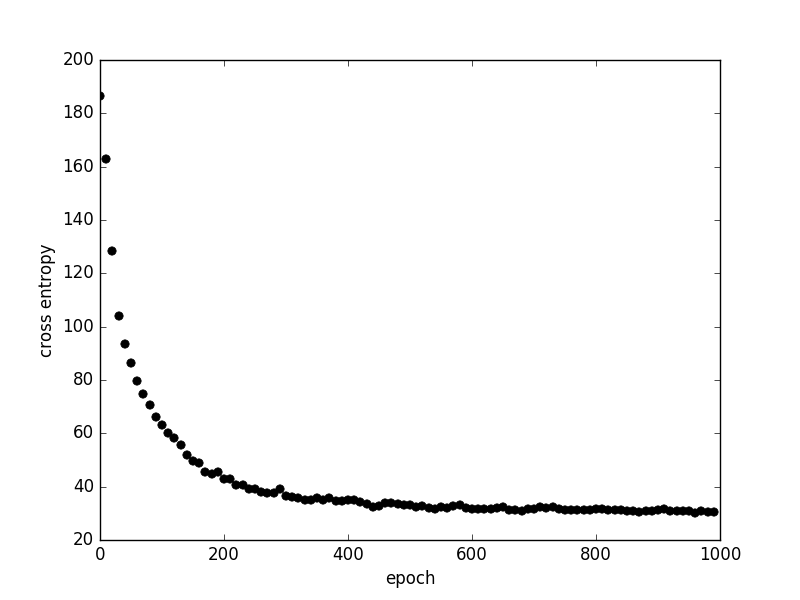
\includegraphics[scale=0.8]{./koki/l.png} \\
   \caption{RBM学習時のエポック数とクロスエントロピーの関係}
\label{fig:ep}
\end{center}
\end{figure}

以上の結果より,クロスエントロピーが確実に収束するエポック数としてエポック数を1000と決定した.

\subsection{出力層の学習率とエポック数}
出力層の学習率とエポック数を決定するため予備実験を行った.文献\cite{Hinton-guide}を参考に更新量が重みの$10^{-3}$程度になるよう決定した.
学習エージェントが実際に採集した,入力を盤面の状態とし,出力を次に石を置く盤面の位置とするデータセットを利用する.
RBMの素子数は\ref{sec:node}で説明した自動決定法により決定した.
エポック数と教師データと出力データの二乗和誤差との関係を以下の図\ref{fig:tu}に示す.

\begin{figure}[]
\begin{center}
   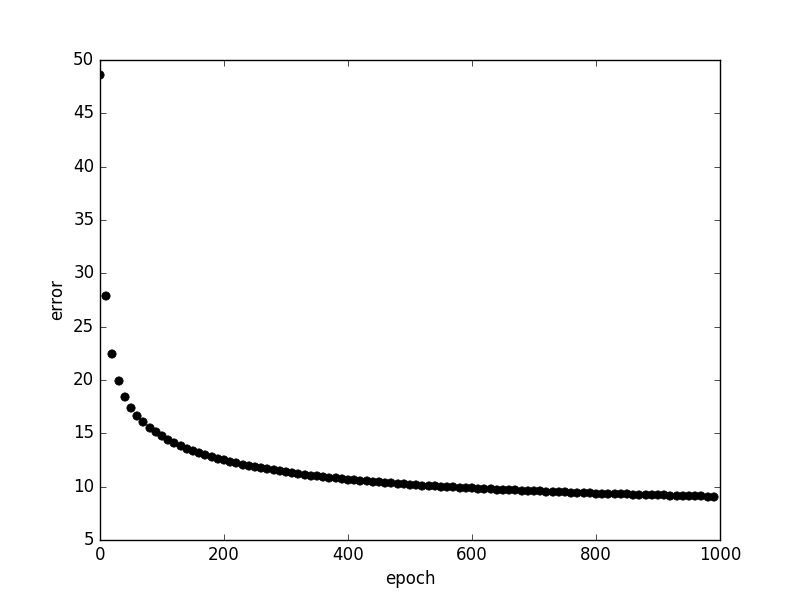
\includegraphics[scale=0.8]{./koki/t.png} \\
   \caption{RBM学習時のエポック数とクロスエントロピーの関係}
\label{fig:tu}
\end{center}
\end{figure}

以上の結果より,二乗和誤差が確実に収束するエポック数としてエポック数を1000と決定した.

\section{提案手法の評価実験}
予備実験にて決定した各種パラメータを用いて,評価実験を行った.

先行に対戦相手のランダムエージェント,後攻に学習エージェントを設定し,三目並べタスクを行った.

三目並べシステム,エージェントの詳細は\ref{ch:ilrbm}にて記述したとおりである.詳細な実験条件を\ref{tbl:exp}に示す.

エージェントは提案手法である負のネットワーク,負のサブゴールを実装したものと,既存手法の負のネットワークを実装していない既存手法\cite{osawa}の二種類を比較した.それぞれのエージェントに対し,勝率,敗北率,引き分け率を調査した.

各ターンごとの勝利数,敗北数,引き分け数を表\ref{tbl:r1},表\ref{tbl:r2}に示す.

\begin{table}[]
\begin{center}
	\caption{実験条件}
	% \ecaption{Experimental Condition}
	\label{tbl:exp}
	\begin{tabular}{|c|c|}
		\hline
		$ 1ターンの試行回数					$	& 4000	\\ \hline
		$ 実験ターン数	$	& 6	\\ \hline
		$ 入力層のノード数 $	& 18	\\ \hline
		$ 出力層のノード数 $	& 9	\\ \hline
		$ RBMの隠れ層の初期ノード数 $& $1$\\ \hline
		$ RBMの隠れ層の追加ノード数		$	& \ref{sec:node}により決定	\\ \hline
		$ RBMの学習率					$	& 0.02	\\ \hline
		$ 出力層のパーセプトロンの学習率 $	& 0.02	\\ \hline
		$ RBMの学習のエポック数 $	& 1000	\\ \hline
		$ パーセプトロンの学習のエポック数 $	& 1000	\\ \hline
	\end{tabular}
\end{center}
\end{table}

\begin{table}[]
\begin{center}
	\caption{提案手法の実験結果}
	% \ecaption{Result (desired value:15.0)}
	\label{tbl:r1}
	\begin{tabular}{|c|c|c|c|c|c|c|}
		\hline
		 ターン数 & 1 & 2 &3&4&5&6\\
		\hline
		勝利数	& 1893 & 2840 & 3004 & 3099 & 3113 & 3118 \\
		敗北数&	1796&956&866&786&744&784 \\
		引き分け数&311&204&130&115&143&98 \\
		\hline
	\end{tabular}
\end{center}
\end{table}

\begin{table}[]
\begin{center}
	\caption{既存手法の実験結果}
	% \ecaption{Result (desired value:15.0)}
	\label{tbl:r2}
	\begin{tabular}{|c|c|c|c|c|c|c|}
		\hline
		 ターン数 & 1 & 2 &3&4&5&6\\
		\hline
		勝利数	& 1628&2696&3003&3114&2885&2825 \\
		敗北数&	2094&1290&947&856&1092&1146 \\
		引き分け数 &278&14&50&30&23&29 \\
		\hline
	\end{tabular}
\end{center}
\end{table}



\begin{figure}[]
\begin{center}
   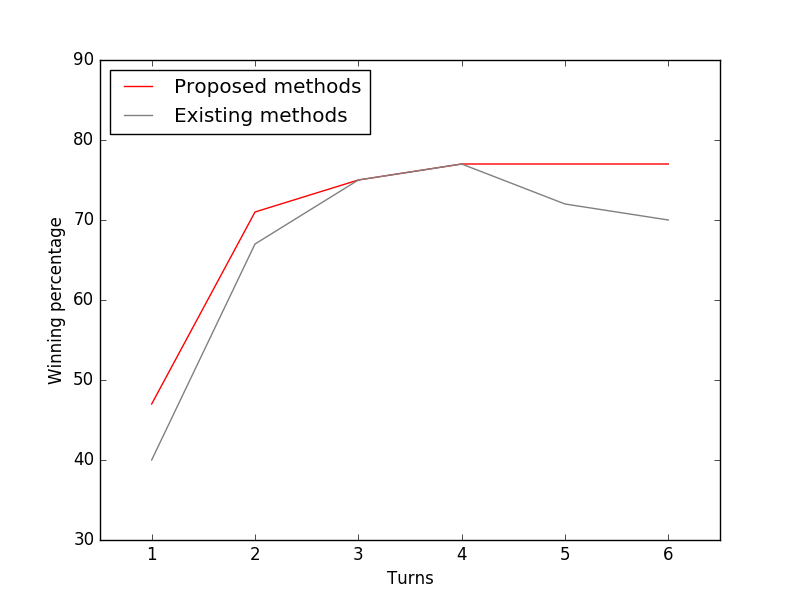
\includegraphics[scale=0.8]{./koki/w.png} \\
   \caption{勝率の比較}
\end{center}
\label{fig:w}
\end{figure}

\begin{figure}[]
\begin{center}
   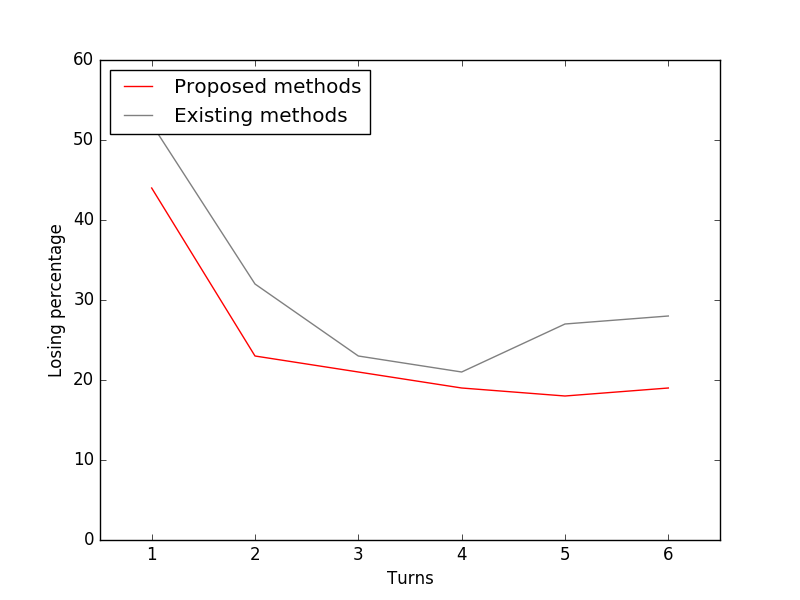
\includegraphics[scale=0.8]{./koki/ll.png} \\
   \caption{敗北率の比較}
\end{center}
\label{fig:ll}
\end{figure}

\begin{figure}[]
\begin{center}
   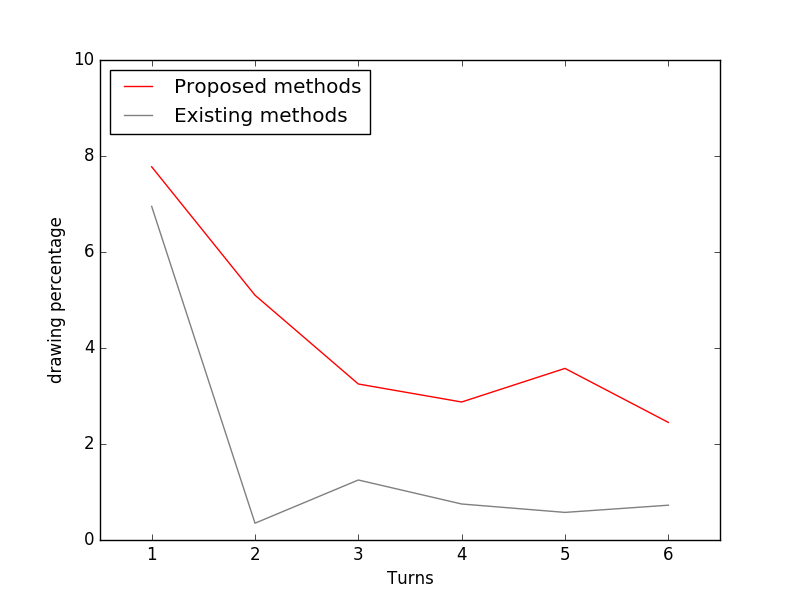
\includegraphics[scale=0.8]{./koki/d.png} \\
   \caption{引き分け率の比較}
\end{center}
\label{fig:d}
\end{figure}

\section{実験結果に対する考察}
図\ref{fig:w}より,提案手法は既存手法に比べ,勝率の点ではほとんど変化が見られず,若干の上昇しか見られなかったものの,図\ref{fig:ll},図\ref{fig:d}より,敗北率の減少と,引き分け率の増加が観察された.

これは,提案手法,既存手法ともに勝利条件に紐づくサブゴールの獲得は共に上手く行っているため,勝率に関しては二手法ともにほとんど変化が見られなかったことが示唆される.
すなわち,現在の盤面が自分に有利な状況,すなわち勝ちにつながりやすい盤面である場合,その盤面の環境を観測してから,勝ち条件をみたすための最適行動を出力する学習は,二手法ともに上手く行っている.

一方,敗北率が減少している点について,提案手法の負のサブゴールの働きにより,上手く敗北濃厚な場面を避けている学習が実現していることがわかる.
既存手法では,敗北を避ける学習を行うことが出来なかった.
三目並べでは,自身が後攻である場合,相手の手によってはどこに打っても勝利盤面へ持っていけない状況が存在する.既存手法では勝利盤面の環境に紐づく盤面しか学習できないため,どこに打っても勝利盤面へ遷移しない状況下において最適行動学習を行うことが出来ない.

一方,提案手法では,敗北時の盤面と紐づく状況も学習することができるため,どこへ打っても勝利に至らない盤面から,敗北を避け,引き分けへと持っていく最適行動が学習できていると考える.

